\documentclass[letterpaper,11pt]{article}

\usepackage{latexsym}
\usepackage[empty]{fullpage}
\usepackage{titlesec}
\usepackage{marvosym}
\usepackage[usenames,dvipsnames]{color}
\usepackage{verbatim}
\usepackage{enumitem}
\usepackage[hidelinks]{hyperref}
\usepackage{fancyhdr}
\usepackage[english]{babel}
\usepackage{tabularx}
\usepackage{fontawesome5}
\usepackage{multicol}
\setlength{\multicolsep}{-3.0pt}
\setlength{\columnsep}{-1pt}
\input{glyphtounicode}

%new packages

\usepackage{fontenc}
\usepackage{amsmath}
\usepackage{amssymb}
\usepackage{graphicx}



%----------FONT OPTIONS----------

\pagestyle{fancy}
\fancyhf{} % clear all header and footer fields
\fancyfoot{}
\renewcommand{\headrulewidth}{0pt}
\renewcommand{\footrulewidth}{0pt}

% Adjust margins
\addtolength{\oddsidemargin}{-0.6in}
\addtolength{\evensidemargin}{-0.5in}
\addtolength{\textwidth}{1.19in}
\addtolength{\topmargin}{-.7in}
\addtolength{\textheight}{1.4in}

\urlstyle{same}

\raggedbottom
\raggedright
\setlength{\tabcolsep}{0in}

% Sections formatting
\titleformat{\section}{
  \vspace{-4pt}\scshape\raggedright\large\bfseries
}{}{0em}{}[\color{black}\titlerule \vspace{-5pt}]



% Ensure that generate pdf is machine readable/ATS parsable
\pdfgentounicode=1

%-------------------------
% Custom commands
\newcommand{\resumeItem}[1]{
  \item\small{
    {#1 \vspace{-2pt}}
  }
}

\newcommand{\classesList}[4]{
    \item\small{
        {#1 #2 #3 #4 \vspace{-2pt}}
  }
}

\newcommand{\resumeSubheading}[4]{
  \vspace{-2pt}\item
    \begin{tabular*}{1.0\textwidth}[t]{l@{\extracolsep{\fill}}r}
      \textbf{#1} & \textbf{\small #2} \\
      \textit{\small#3} & \textit{\small #4} \\
    \end{tabular*}\vspace{-7pt}
}

\newcommand{\resumeSubSubheading}[2]{
    \item
    \begin{tabular*}{0.97\textwidth}{l@{\extracolsep{\fill}}r}
      \textit{\small#1} & \textit{\small #2} \\
    \end{tabular*}\vspace{-7pt}
}

\newcommand{\resumeProjectHeading}[2]{
    \item
    \begin{tabular*}{1.001\textwidth}{l@{\extracolsep{\fill}}r}
      \small#1 & \textbf{\small #2}\\
    \end{tabular*}\vspace{-7pt}
}


\newcommand{\resumeSubItem}[1]{\resumeItem{#1}\vspace{-4pt}}

\renewcommand\labelitemi{$\vcenter{\hbox{\tiny$\bullet$}}$}
\renewcommand\labelitemii{$\vcenter{\hbox{\tiny$\bullet$}}$}

\newcommand{\resumeSubHeadingListStart}{\begin{itemize}[leftmargin=0.0in, label={}]}
\newcommand{\resumeSubHeadingListEnd}{\end{itemize}}
\newcommand{\resumeItemListStart}{\begin{itemize}}
\newcommand{\resumeItemListEnd}{\end{itemize}\vspace{-5pt}}


\begin{document}
\begin{center}
\parbox{3.0cm}{%
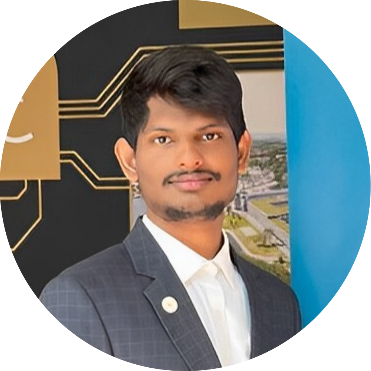
\includegraphics[width=2.7cm,clip]{images/resume_pic_m.png}}
\parbox{\dimexpr\linewidth-3.8cm\relax}{
\vspace{-20pt}
\begin{tabularx}{\linewidth}{L r} \\
    {\Huge \scshape Venkata Sai Yakkshit Reddy Asodi}~ \href{https://www.cedzlabs.com/yakkshit}{\vspace{1pt}}\\
      Berlin, Germany. \\ \vspace{1pt}
     \small \raisebox{-0.1\height}\faPhone\ +91 8179936156 ~ \href{mailto:saiyakkshit2001@gmail.com}{\raisebox{-0.2\height}\faEnvelope\  {saiyakkshit2001@gmail.com}} ~ 
    \href{https://linkedin.com/in/yakkshit/}{\raisebox{-0.2\height}\faLinkedin\ {yakkshit}} ~
    \href{https://yakkshit.com/}{\raisebox{-0.2\height}\faGlobe\ {yakkshit.com}} ~
    \href{https://github.com/yakkshit}{\raisebox{-0.2\height}\faGithub{ yakkshit}}
    \vspace{-8pt}
\end{tabularx}
}
\end{center}

\vspace{-20pt}
\section{Summary}
Dynamic Frontend Developer with over five years of experience building intuitive, accessible web applications using React and TypeScript. Proven expertise in delivering scalable and user-friendly designs, especially in agile environments. Passionate about utilizing technology for social good, with a focus on empowering communities through digital platforms. Adept at translating team discussions into fully functioning applications with a strong emphasis on usability and accessibility.

\section{Technical Skills}
\begin{itemize}[leftmargin=0.15in, label={}]
\small{\item{
\textbf{Frontend:} React, TypeScript, JavaScript (ES6+), HTML5, CSS3, Emotion (CSS-in-JS) \\
\textbf{Backend:} Node.js, Express, RESTful APIs \\
\textbf{Tools:} Git, Docker, Kubernetes, GitFlow, Postman, Swagger \\
\textbf{Testing:} Jest, Cypress, E2E Testing, Unit Testing \\
\textbf{Deployment:} AWS, Azure, CI/CD Pipelines, Kubernetes, Docker \\
}}
\end{itemize}
\vspace{-10pt}

\section{Experience}
\resumeSubHeadingListStart
\resumeSubheading
{\large Circleup AG}{December 2023 -- July 2024}
  {Lead Full Stack Engineer (Frontend Focus)}{Zurich, Switzerland}
\begin{itemize}
    \item Led the development of responsive web applications, translating designs into user-friendly React and TypeScript interfaces.
    \item Collaborated on feature planning and architecture decisions, optimizing accessibility and usability across platforms.
    \item Developed reusable components, contributing to the design system and ensuring code consistency across teams.
\end{itemize}

\resumeSubheading
{Cedzlabs}{March 2023 -- July 2024}
{Full Stack Developer (Frontend Focus)}{India}
\begin{itemize}
    \item Worked on UI/UX development, ensuring accessibility and responsive design in collaboration with designers and engineers.
    \item Integrated APIs into React applications, focusing on seamless user interactions and optimized performance.
\end{itemize}

\resumeSubHeadingListEnd

\section{Projects}
\resumeProjectHeading
{\textbf{Social Campaign Platform} $|$ \emph{React, Node.js, TypeScript}}{January 2024}
\begin{itemize}
    \item Developed a web platform for social campaigns, allowing users to create and sign petitions, with full internationalization support.
    \item Integrated user authentication, petition tracking, and campaign sharing via REST APIs.
    \item Built reusable components with a focus on accessibility, ensuring WCAG compliance and intuitive user navigation.
\end{itemize}

\resumeProjectHeading
{\textbf{AI Resume Tuner} $|$ \emph{Azure Cloud, Next.js, LLMs}}{August 2023}
\begin{itemize}
    \item Developed a tool for generating tailored resumes using AI, integrating Retrieval-Augmented Generation (RAG) and LLMs.
    \item Built the frontend with Next.js, providing a smooth user experience and secure data handling on Azure Cloud.
\end{itemize}

\resumeProjectHeading
{\textbf{Portfolio Website} $|$ \emph{NextJS, AWS}}{January 2023}
\begin{itemize}
    \item Created a secure, scalable portfolio website using NextJS and AWS, highlighting personal projects and achievements.
    \item Focused on responsive design and optimized performance for web and mobile devices.
\end{itemize}

\section*{Languages}
\begin{itemize}
  \item Telugu - Native $|$ English - Fluent $|$ Hindi - Fluent $|$ German - Elementary $|$ Swedish - Elementary.
\end{itemize}

\section{Achievements}
\begin{itemize}
    \item Contributed to open-source projects focused on accessibility and component-based design systems.
    \item Led UI/UX development workshops at tech meetups, sharing best practices for React and TypeScript.
    \item Active participant in social impact initiatives, helping develop digital tools for community organizing.
\end{itemize}
\end{document}